\documentclass[oneside]{article}
\usepackage[a4paper,left=1in, right=1in,
                   showframe=false]{geometry}
\usepackage{graphicx,xcolor}
\usepackage{verse,picture}
\pagestyle{empty}
\parindent0pt
\parskip0pt
\makeatletter
\newif\if@debug
\@debugtrue
%\@debugfalse % comment to see rules and boxes
\if@debug
   \fboxrule0.4pt
   \fboxsep0.2pt
   \def\rulecolor{orange}
\else
   \fboxrule0pt
   \fboxsep0pt
   \def\rulecolor{white}
\fi
\def\Rule#1#2{%
  {\color{\rulecolor}
  \rule{#1}{#2}}
}
\def\floatright{\dimexpr\textwidth-80pt\relax}
\def\floatleft{0pt}
\makeatother
\settowidth{\versewidth}{And the bright morning dew is his meat}
\begin{document}
\Rule{5pt}{60pt}

\fbox{\vbox{\poemtitle*{THE BEETLE}}}
\Rule{15pt}{53pt}
\Rule{15pt}{3pt}{\fbox{\vbox to 0pt{%
          % \fbox{%
           \Rule{\floatright}{5pt}%
           \begin{picture}(0,0)
           \put(-13cm,-5cm){\hbox{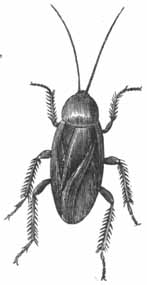
\includegraphics[width=80pt]{beetle}}}
           \end{picture}
         %}%
}}}
%}

\begin{verse}[\versewidth]
See the beetle that crawls in your way,\\
\vin And runs to escape from your feet;\\
His house is a hole in the clay,\\
\vin And the bright morning dew is his meat.\\
\bigskip
But if you more closely behold\\
\vin This insect you think is so mean,\\
You will find him all spangled with gold,\\
\vin And shining with crimson and green.\\
\bigskip
Tho' the peacock's bright plumage we prize,\\
\vin As he spreads out his tail to the sun,\\
The beetle we should not despise,\\
\vin Nor over him carelessly run.\\
\bigskip
They both the same Maker declare---\\
\vin They both the same wisdom display,\\
The same beauties in common they share---\\
\vin Both are equally happy and gay.\\
\bigskip
And remember that while you would fear\\
\vin The beautiful peacock to kill,\\
You would tread on the poor beetle here,\\
\vin And think you were doing no ill.\\
\bigskip
But though 'tis so humble, be sure,\\
\vin As mangled and bleeding it lies,\\
A pain as severe 'twill endure,\\
\vin As if 'twere a giant that dies%
\footnote{Anonymous, \textit{Illustrared London Book} 1851.}%
\footnote{Note that all lines start with a capital letter. 
This follows English tradition, but modern poetry is not always capitalized.}.\\
\end{verse}
\end{document}

Change floatright to floatleft to see how the image moves from left to right.


I am interested to see how this is handled in LaTeX3 or alternative solutions in LaTeX (not using put or TikZ). 

